\chapter{Exploring The Feasibility of Comparing Software Components}
\label{chapter:fs1}

This chapter investigates the challenges of identifying, selecting, and comparing ostensibly similar software components. A feasibility study was created to compare the performance (speed) of a cohort of text template engine components and the results were analysed.

\section{Introduction}
\label{fs1:intro}

In principle, whenever the decision is made to include external libraries, components, or applications in a software product, component sources and candidates should be investigated, evaluated, and compared in order to make a final decision. In practice, things are much more complex than this \citep{Badampudi2016}. The literature contains many attempts to rationalise and streamline this process, using approaches such as economic models \citep{Milkman2009}, \enquote{decision maps} \citep{Lago2019} and even machine learning \citep{Maxville2004}.

A typical component selection process consists of several broad phases: \emph{discovery} of the potential candidates, \emph{filtering} by eliminating clearly inappropriate candidates, and \emph{evaluation} of the remainder to determine their suitability. These phases may be sequential, or they may overlap, but in principle each candidate component passes through the process.

There is no single `catalogue' of software to choose from, so even discovering a list of potential sources or candidates can be time-consuming and will probably be incomplete. Open source software components are available from a wide range of sources including: general code repositories such as \emph{GitHub}\footnote{\url{https://github.com/}}, \emph{Bitbucket}\footnote{\url{https://bitbucket.org/}}, \emph{Sourceforge}\footnote{\url{https://sourceforge.net/}}, and \emph{Google Code}\footnote{\url{https://code.google.com/}}; organisation-specific repositories such as \emph{The Apache Projects Directory}\footnote{\url{https://projects.apache.org/}}; and language-specific package repositories such as \emph{Maven Central}\footnote{\url{https://repo.maven.apache.org/maven2/}}, \emph{CPAN}\footnote{\url{https://www.cpan.org/}}, and \emph{PyPi}\footnote{\url{https://pypi.org/}}. These repositories are not exclusive - some software components may appear in multiple repositories. Software components are also not entirely distinct. Popular open source software components are often `forked', a process roughly equivalent to copying and modifying, so similar components may appear in multiple repositories with different names and potentially different features, bugs, and non-functional attributes.

Most repositories provide basic programming language and operating system compatibility information, so filtering candidates at that level is relatively simple. Beyond that, filtering relies on the documentation (including the source code, if available) provided for the component. However, documentation for software varies widely in content and structure and is often biased, incomplete, or inaccurate \citep{Bertoa2003}. Further filtering requires a mixture of investigating the documentation provided with the component and exploring other sources of information such as external reviews, articles, and comparison websites.

Evaluation of software components can be lengthy and expensive, particularly when the requirements for the component are complex or there are large numbers of candidates to choose from \citep{Badampudi2016}. In many cases components will not be directly interchangeable, but require software to be written or changed in order to use them. This adds time and cost to any kind of in-situ comparisons.

Where time and cost are important, as they almost always are, it is common to resort to heuristics based on factors such as personal experience, project or company history, or what has been read about recently. In many cases the evaluation process will stop as soon as a candidate is encountered which appears functionally suitable. What is rarely apparent is how much candidates may differ in `non-functional' aspects such as performance, maintainability, and energy efficiency. This chapter will explore this issue through the lens of one particular type of software component: the \emph{template engine}.

\subsection{Templates and Template Engines}

In the early days of computing the emphasis was largely on numerical calculations. The term `computer', was originally a job title for someone who performed calculations rather than a machine \citep{NASA2016}. Despite this, there has always been a strand of computing which deals with text. Some of the earliest electronic computers were used for code-breaking of textual messages \citep{Copeland2004}.  Almost every modern use for computers has a need to produce textual output, even if just for error messages or activity logs. 

Text output may be produced in a range of ways. The simplest is probably direct output of `strings', quoted blocks of text hand-crafted by software developers, included in the text of a program. Another option is loading and output of pre-generated blocks of text from storage such as a file or a database. Some text output, however, needs to include information which was not known when the software or the stored data was created. In such situations what is needed is a combination of fixed text and variable content: \enquote{a dynamic and computational text} \citep{Rodgers1999}. As an example, most business software comes with some sort of `mail merge' facility to produce form letters with a bit more individuality than `\emph{Dear customer ...}'.

One way to produce such dynamic text is to generate it in stages, creating a sequence of fixed and variable parts which have the appearance of a single document. This approach is typically done in-line within the software, which can make it relatively simple to create and generally fast in execution. However, text generated in this way can be difficult to maintain as it requires updating the software for every change, and including large blocks of static text in program code can be cumbersome. In-line text generation is usually restricted to small or single-use software.

The most common method for producing these kinds of documents uses a \emph{templating} technique. A \emph{template} is a document containing both fixed text and special symbolic tokens, known as \emph{placeholders} \citep{Arnoldus2007}. To generate a document a template is processed using a type of software known as a \emph{template engine}, which replaces the placeholders with stored or calculated data to generate individualised output documents.

Templating is not limited to personalised mail. A similar approach produces a \enquote{substantial fraction} of the visible pages of the web \citep{Yang2008}. In 2005 \citeauthor{Gibson2005} estimated that

\begin{displayquote}
Templates represent 40–50\% of the total bytes on the web, and this fraction continues to grow at a rate of approximately 6\% per year.
\end{displayquote}

\citeauthor{Gibson2005}'s study is relatively old in technology terms, however. The estimated growth has clearly not continued or by now there would be more templated content than the web itself! However, the enormous growth of the web since that study has made the determination of such estimates considerably more difficult particularly if attempting to use the technique employed by \citeauthor{Gibson2005}, which relied on statistical analysis of a `snapshot' of \emph{the whole web}. Despite examining over 250 papers which cite \citeauthor{Gibson2005}, up to and including 2023, no better estimates have yet been found.

Templated text generation is also common in much of the less visible internet traffic. Emails and other textual messages, logging, diagnostic output, code generation \citep{Fritzson2009} \citep{Arnoldus2010} and a wide variety of formats and protocols \citep{Barbosa2002}, all benefit from this powerful technique.

Proceeding on the assumption that templated content comprises at least \citeauthor{Yang2008}'s  `substantial fraction' of the web and considering the web size estimates from \citet{Worldwidewebsize2018} and \citet{Kunder2008}, it seems fair to assume that template-generated web pages number in the billions. Public website visits range from single figures to hundreds of thousands or even millions per month \citep{Castillo2023} which implies that the overall number of template pages generated is probably at least trillions per month. The impact of even small differences in performance and energy usage of template engine software could therefore be huge.

\subsection{Template Engine Software}

Unfortunately, there is little consensus in this field. A template engine is a conceptually simple piece of software, sometimes used as a teaching aid \citep{Koskela2007}, but which has the potential for many different implementations with different features and complexity. A search of the popular open source software website \emph{GitHub} \citep{GitHubGeneral} reveals over 13,000 software projects with names or descriptions which include the term `template engine' (\autoref{github}). A cursory examination of the results indicates that the great majority of these results are separate template engine implementations in some state of development as mentioned in \autoref{fs1:intro}. GitHub is not the only source of software components and libraries. Selecting a template solution for a project can be a major task.

\begin{figure}[ht!]
\centering
\includegraphics[width=\columnwidth]{Figures/template-engines-2023.png}
\caption{GitHub search for the term `Template Engine' in October 2023}
\label{github}
\end{figure}

Comprehensive comparative information about the many differing implementations can be hard to come by. Software documentation for such tools, where present at all, tends to focus on the use of a single implementation and often reads more like marketing material than a datasheet: emphasising strengths with unverified claims, ignoring weaknesses, and avoiding direct comparison with alternatives.

Template technology is therefore a representative category of software implementation which exhibits the scale, consequences, and lack of easy choices discussed in \autoref{section:motivation summary}. The rest of this chapter will dig deeper into template technology, its characteristics, and the variation between a range of implementations.

\subsection{Concepts and Terminology}

There are several key concepts which inform this research. The intention is to explore these in detail in further sections, but for now, some non-definitive descriptions:

\begin{description}
\item[Template] 

A template is a way of ensuring consistency and reducing re-typing when creating similar documents. Common text and layout are entered just once and then reused to produce many pages or documents. Each template is described in terms of a specific \emph{template language} and designed to be rendered by a compatible \emph{template engine}.

\item[Template Engine] 

A template engine is a software system or component which manages the rendering of \emph{templates}. When an output document is required, the template engine locates an appropriate \emph{template}, loads the data for the desired document into a \emph{page context}, then processes the template by interpreting it according to the \emph{template language} and replacing \emph{placeholder expressions} with appropriate data from the \emph{page context}. 

\item[Template Language] 

A template language specifies how a \emph{template} is expressed. Most template languages consist of a combination of fixed text ready for output (known as `\emph{boilerplate}') and symbolic placeholders. Some template languages use symbolic expressions for everything, including fixed text. Template languages and their placeholder expressions vary widely, but within many template languages it can be useful to consider two types of placeholders: \emph{value expressions} and \emph{control expressions}.

\item[Value Expression] 

A value expression is a sequence of symbols representing the name or location of a data value. When the template is rendered, the value expression will be replaced by a textual version of the data value. If the data value is already textual it will usually just be included in the output. If the data value is numeric or some more complex data type, the way it is rendered will depend on the \emph{template engine} and any options specified in the value expression. The details of the formatting and syntax of such expressions are specified as part of the \emph{template language}.

\item[Control Expression] 

A control expression is not directly replaced by a value in the rendered output, but instead informs the process of rendering the template. Typical control expressions mimic those of conventional programming languages and include, for example: variables, decisions, and loops. Others may have side-effects specific to a particular \emph{template engine} or \emph{template language}.

\item[Page Context] 

A page context is the way that a \emph{template engine} finds data to use when processing \emph{value expressions}. Most \emph{template engines} treat the page context as if it is a simple named data store containing everything needed by the \emph{value expressions} in the \emph{template} currently being processed. However, page context implementations are also available which do not pre-load data before evaluating the \emph{template}, but instead load or calculate data as needed during the processing of the \emph{template}. As each rendered document will potentially be different, a new page context is provided for each document, and the rendering process evaluates the \emph{template} using the specific data from that page context. Depending on the strategy used by the \emph{template engine}, the \emph{template} to use for each document may be determined by examining the page context, or it may be specified externally.

\end{description}

More details of the capabilities and characteristics of template languages and template engines are explored in \autoref{chapter:intermediate}.

\subsection{Templating in the Literature}

There is a substantial body of literature which mentions some form of templating in passing, either philosophically \citep{Bush1945} \citep{Nelson1974} or as a means to achieve a specific end \citep{Caldwell1998} However, while these may contain some information about the selection and use of templating systems, they are not the core of this research. The pool of literature which directly addresses theory and implementation of templates and template languages seems much smaller.

Grouping and categorising is a key way to advance knowledge. \citet{Vegas2009} assert that in science and engineering, knowledge matures as the investigated objects are classified. With the rise in popularity of template approaches, particularly when used to generate web pages, some effort has been put into trying to group template languages and/or template engines into categories to build a body of knowledge and determine unifying constructs; interrelationships; and knowledge gaps \citep{Vegas2009}, with which to reason about capabilities and applicability for different kinds of usage.

\citet{Vosloo2008} set out to survey and classify the landscape of server-side web page generation frameworks. Tellingly they were unable to find other literature at this level of detail:

\begin{displayquote}
This proliferation of discussions and solutions may be construed as an indication that the problem (of finding the right abstractions with which to implement Web-based UI) has not been solved satisfactorily in practice. However, it may also be that the problem merely has a great number of variable parts, and that it needs to be partitioned more usefully. \citep{Vosloo2008}
\end{displayquote}

\citeauthor{Vosloo2008} initially divide the web page technologies they examine according to the three aspects of the popular MVC (Model, View, Controller) pattern. Their research is primarily concerned with what \citeauthor{Vosloo2008} describe as \enquote{view concerns}. They consider possible taxonomies of page-generation strategies including various forms of templates, eventually presenting the diagram shown in \autoref{diagram:vosloo2008}.

\begin{figure}[ht!]
\centering
\includegraphics[width=130mm]{Figures/taxonomy.png}
\caption{A Taxonomy of Strategies for View Concerns from \citet{Vosloo2008}}
\label{diagram:vosloo2008}
\end{figure}

The final paragraph of \citet{Vosloo2008}'s \enquote{view concerns} section highlights the usefulness of taxonomy construction in finding under-considered areas:

\begin{displayquote}
For example, none of the 80 frameworks studied relied on a template language with the same basic goal of the page composition variants (Section 5.8), but with a syntax external to the host markup language. ... The absence of such a category in the aforesaid taxonomy could perhaps be the trigger for developing just such a language. \citep{Vosloo2008}
\end{displayquote}

There are, however, two key issues with \citeauthor{Vosloo2008}'s approach. The first is that only server-side web frameworks were considered for the study. While this does not invalidate their results, it does imply that the classification work would need to be re-done if page-generation tools in other technologies, or template techniques for non-web uses were to be included.

Another issue is a more general one with all such taxonomies. As pointed out by \citet{Usman2017} \enquote{most taxonomies are developed in an ad-hoc way}, and \enquote{taxonomies are rarely revisited, revised or extended}. New server-side frameworks and template technologies are continually being produced, and existing ones are continually being revised, updated and re-released. A several-year-old ad-hoc summary is likely to be neither exhaustive nor fully correct and should be considered as a historical source rather than a complete reference. Even with this caveat, though, \citeauthor{Vosloo2008}'s list of 86 server-side web frameworks, most of which have at least some template processing features, begins to show the scale of the problem.

\citet{Laakso2008} also attempt to categorise a selection of web frameworks. As seen in \citet{Vosloo2008}, web frameworks often have template features. \citet{Laakso2008} also have trouble finding prior work on which to base their research:

\begin{displayquote}
To the best of authors' knowledge, very little research has been done about measuring web application frameworks. \citep{Laakso2008}
\end{displayquote}

They do, however, recommend two articles: \citet{Zoio2005} and \citet{Kolesnikov2006}. \citeauthor{Zoio2005} presents a detailed and practical comparison between two frameworks: \emph{JSF}\footnote{\url{https://www.oracle.com/java/technologies/javaserverfaces.html}} and \emph{Tapestry}\footnote{\url{https://tapestry.apache.org/}} through the approach of building the same application twice, once in each of the two competing technologies. \citeauthor{Kolesnikov2006} describes the use of Tapestry in an MSc dissertation.

\citet{Laakso2008} take an experimental approach, as does \citet{Zoio2005}. Both design one or more scenarios, apply them to each of the implementations, and use the results to measure the suitability of different software systems. The comparisons generally concentrate on ease of development and deployment, although there is some mention of rendering performance, which may be analogous to efficiency, and thus affect resource usage. 

Concentrating more specifically on templates, \citet{Parr2004} sets out to 

\begin{displayquote}
formalize the study of template engines, thus, providing a common nomenclature, a means of classifying template generational power, and a way to leverage interesting results from formal language theory. \citep{Parr2004}
\end{displayquote}

\citeauthor{Parr2004}, however, presents the opinion that a template is a pure and separate view and should be "totally divorced from the underlying data computations whose results it will display" (ibid p2) While this is arguably a justifiable position, it does lead to a taxonomy which essentially has two categories: those which enforce such separation, and those which do not. The fully separated category mainly consists of a new template language, \emph{StringTemplate}\footnote{\url{https://www.stringtemplate.org/}}, developed alongside the paper, with almost every other solution relegated to `do not'. \citeauthor{Parr2004} also limits his discussion to template-style solutions written in the Java programming language.

Although \citeauthor{Parr2004}'s \emph{StringTemplate} language has been used for other academic publications \citep{Fritzson2009} \citep{Arnoldus2010} \citep{Hartmann2011} \citep{Arnoldus2012} \citep{Vollebregt2012} and many more, Parr admits that commercial programmers often prefer the features of other, less pure but more powerful, template languages. Implicitly, therefore, there is still a need to categorise these other template languages beyond simply whether or not they enforce separation.

\citet{Arnoldus2010} also addresses the language used in templates, but from a grammatical perspective. The important categorisation distinction in Arnoldus’ work is that of `safety'. Having determined that \enquote{Writing templates, and code generators in general, is a complex and error prone task} (p103), Arnoldus introduces the concept of a `syntax-safe' template, which is incapable of generating grammatically incorrect output. This is particularly important when the output is intended to be machine readable, with a formal grammar, and Arnoldus concentrates on the specific application area of program generation, which exhibits these characteristics. Although Arnoldus does not attempt a categorisation of template languages, he does discuss several key factors (such as the presence of `hedges' (p111), separating placeholder expressions from other text) which are commonly found in those template languages which are more suitable for syntax-safe applications.

\subsection{Discussion}

Templates are the technology of choice for a large proportion of the world's web pages, and thus it seems plausible that the generation of these pages contributes in some part to the large energy and resource usage of the internet and the world wide web.

While there has been some consideration of template engines and template languages in academic literature, the quantity of such papers is dwarfed by the number of software implementations, websites and documentation which have not been through any form of academic peer review process. Template engines and template languages vary widely. Attempts have been made to construct taxonomies in related fields such as web applications, and crowd-sourced information is available from sources such as Wikipedia, but so far, no sign has been found of a detailed and comprehensive comparison and analysis of a wide range of template engine implementations. In the context of this research, so far no taxonomies have been found which include or mention energy consumption, energy-efficiency, or resource usage in general.

It would seem, therefore, that there is an opportunity for research in this field to contribute to knowledge and thereby to potentially assist in improving the overall resource usage of large software systems.

\section{Methodology}
\label{fs:methodology}

Even though there are several implementations of template engines mentioned in the literature, there are also many more available. Rather than attempt to gather detailed information about every possible software candidate before starting, the intention was to proceed incrementally, building a collection of data on a growing subset, using preliminary analysis and reflection to inform further research.

Before embarking on a potentially lengthy experimental process, it seemed prudent to attempt to determine whether such research would be likely to provide interesting results. The overall research goal was to help software developers make informed choices to minimise the environmental impact of their work. If measurable differences could be found even between a small selection of software components, then component selection or substitution could be a valid environmental strategy.

With thousands of template engines to choose from, the scope of any initial feasibility study needed to be constrained. Options included limiting the study by popularity, by application domain, by the preferences of specific software developers, by programming language, by template language, by price, or many other factors. Each of these options had theoretical advantages and disadvantages. However, an initial feasibility study needed to be practical and provide results as soon as possible. Following the approach used by \citet{Laakso2008} and \citet{Zoio2005} a study was planned which would select a small number of template components and construct a software test harness to run an identical set of tests on each of the components. There was no attempt to be exhaustive with the selection of components to test.

The aims of the feasibility study were twofold: to ascertain if this would be a reasonable and useful approach for identifying and comparing template components, and to establish the scale of the variability in features and performance between a sample of available components. Throughout the construction of the study, efforts were made to avoid or constrain `scope creep' \citep{Heinze2014}.

\subsection{Selection of a Programming Language}

To obtain results which could more easily be compared, it was decided to limit the feasibility study to include only template systems in a single programming language. The language \emph{Java} \citep{Oracle2018Java} was chosen for several reasons. Java is generally considered to be one of the most popular programming languages in the world \citep{Tiobe2018}. Java is freely available and runs on a wide range of hardware platforms. Java development tools are also available at University of Suffolk and familiar to the researcher, reducing both the need for training before commencing the study and the risk of mistakes or misunderstandings.

\subsection{Selection of Template Engines}

The next stage was to select an initial set of template engines for the feasibility study. \emph{StringTemplate}\footnote{\url{https://www.stringtemplate.org/}} has been cited several times in academic literature; \emph{Velocity}\footnote{\url{https://velocity.apache.org/}} and \emph{FreeMarker}\footnote{\url{https://freemarker.apache.org/index.html}} are popular in lists of Java template engines on the web \citep{Dzone2016}; \emph{Mustache}\footnote{\url{https://mustache.github.io/}} is probably the most widely implemented style of template engine, with implementations in at least 45 Languages. Four further template engines \emph{Casper}\footnote{\url{https://code.google.com/archive/p/casper/}}, \emph{Hapax}\footnote{\url{https://code.google.com/archive/p/hapax/}}, \emph{Jangod}\footnote{\url{https://code.google.com/archive/p/jangod/}} and \emph{JMTE}\footnote{\url{https://github.com/HubSpot/jmte}} were included, as they take somewhat differing approaches compared to the systems mentioned above.

Two further template engines (\emph{Stringtree}\footnote{\url{https://github.com/efficacy/stringtree}} and \emph{Solomon}\footnote{\url{https://bitbucket.org/efficacy-misc/emo/src/master/src/main/java/org/stringtree/solomon/}}) were included as a baseline for comparison. Both these implementations resulted from previous personal research in this area and so provided familiar implementations to use when developing experiments and test harnesses.

\subsection{Construction of a Feasibility study}

Keeping the feasibility study aims in mind, the following eight simplified \enquote{real world} evaluation scenarios were constructed:

\begin{description}
\item[Scenario S0: No substitutions (`control' case)] \hfill

The job of a template engine is to read and combine a template with some variable data by replacing placeholders. However, not all template documents contain placeholders. Some are just documents to be served unchanged. The processing within the template engine will likely add some overhead. This scenario gives some indication of the processing overhead in each implementation.

\item[Scenario S1: A single textual substitution] \hfill

The simplest active case for a template engine is the identification of a placeholder and its replacement with a single constant textual value. The purpose of this scenario is to evaluate the performance of this common activity.

\item[Scenario S2: A collection of textual values] \hfill

A step up from a single value is the substitution of a collection (such as an array, a list, or some other iterable object) of textual values. This scenario requires the template engine to determine in some way that the value to be substituted is a collection, and to make some attempt at rendering the contents in order.

\item[Scenario S3: A collection separated by commas] \hfill

It is usual in English when presenting a list to separate the items with commas. Given the list (\emph{ham} \emph{eggs} \emph{chips}) it might be typical to present it as \texttt{ham, eggs, chips} (or even \texttt{ham, eggs, and chips}, but that is less common in dynamically generated documents, and beyond the scope of this feasibility study). This scenario is an interesting challenge for a template engine, which is why it is a separate test from simply rendering the contents of a collection. Some template engines make it difficult to avoid placing an excess comma after the final item, for example.

\item[Scenario S4: Include another template] \hfill

Structural Decomposition (colloquially known as \emph{divide and conquer}) is a key practice of software engineering, and also applies to the design and construction of documents such as web pages from component parts. For this to work, a template system must be able to include within its output the result of processing another template. This scenario evaluates the effectiveness of a template engine at constructing compound documents.

\item[Scenario S5 and S6: Show a value if a boolean value is \emph{true} or \emph{false}] \hfill

Conditional execution is another key aspect of software. In the case of template processing it is a common requirement to show a true/false value from the data as text. From a single letter or a glyph such as an emoji or checkmark (\checkmark) to a swathe of boilerplate or a whole extra template, the process is the same. If the value is true, show the specified text. Some template languages make a big issue of the difference between showing some text if true, but nothing at all if false, and showing alternative text such as \checkmark for true and $\times$ for false. These scenarios evaluate the effectiveness of a template system at converting boolean values.

\item[Scenario S7: Call some code] \hfill

Although \citeauthor{Parr2004} considers this a \enquote{violation} of the principle of separation of logic from display, many template systems support the execution of arbitrary code during the rendering of templates. Techniques for achieving this vary widely, but with the Java ecosystem there is a standard way of invoking code from other contexts: the \emph{JavaBeans} API \citep{Oracle2018JavaBean}. Use of this API allows systems such as template engines to execute an object method by treating it as accessing a data field. Typical uses for this facility in a template is to include data which is expensive to pre-calculate or may not be known in advance. This scenario evaluates the effectiveness of a template system at using the \emph{JavaBeans} API.

\end{description}

\subsection{Implementation of a Feasibility Study}

One of the characteristics which separates template systems is the variation in their template languages. An implication of this is that templates cannot usually be re-used to evaluate different template engines. These distinctions are explored in more detail in \autoref{chapter:intermediate}. Likewise, template engines provide a variety of software interfaces.

For best compatibility of test results tests should be as similar as possible, yet the nature of the different template engines requires many differences in implementation. To resolve these tensions, an architecture was chosen which used the strategy pattern \citep{Gamma1994} to enable isolation of specific differences between the code for the various template engines.

\begin{figure}[ht!]
\centering
\includegraphics[width=130mm]{Figures/classes.png}
\caption{Class diagram showing use of strategy pattern}
\label{fs:figure:strategy}
\end{figure}

As each concrete strategy class was coded and tested, it was integrated with a test harness written using the JUnit test library\footnote{\url{https://junit.org/}}. When all implementations were complete, code was added to compare generated output with expected output from each test for each test harness, and to time multiple runs of each such test. Tests were timed using the Java \texttt{System.currentTimeMillis()} method, which uses the system `wall clock' rather than attempting to measure only time used by specific processes or threads.

The code for the test harness underwent several changes as the template implementations were added. Most commonly this was due to differing assumptions between implementations. For example, many template engines expect to fetch templates from a local file system but some prefer other means, so the abstract definition of the strategy implementations had to change to support a wider variety of such sources. As much as possible, however, such changes were kept in the common part of the code rather than being duplicated in template-specific classes.

Despite copious reading of documentation, source code and web articles, it was not possible to coerce all template engines to generate the correct output for all test scenarios. Such failures are noted in the results but it was decided not to exclude these test scenarios from the timed tests.

As testing progressed it became apparent that performance of the differing template engines varied widely, so the timed part of the experiment was tuned to give all the template engines a chance to complete in a reasonable time. Eventually a value of 10,000 repetitions was settled on as an effective number. This gave largely repeatable results for each template engine.

\section{Results}
\label{fs:results}

The success of the test scenarios is given in \autoref{fs:table:features}, and the timings for 10,000 runs of each scenario are given in \autoref{fs:table:times}.

\begin{table}[ht!]
\fontsize{9}{11}\selectfont
  \begin{center}
    \begin{tabular}{r|l|l|l|l|l|l|l|l}
      & {\rotatebox{90}{{\textbf{S0 No Subst}}}} 
      & {\rotatebox{90}{{\textbf{S1 Single Text}}}} 
      & {\rotatebox{90}{{\textbf{S2 Collection}}}}
      & {\rotatebox{90}{{\textbf{S3 Separated}}}}
      & {\rotatebox{90}{{\textbf{S4 Include}}}}
      & {\rotatebox{90}{{\textbf{S5 Bool True}}}}
      & {\rotatebox{90}{{\textbf{S6 Bool False}}}}
      & {\rotatebox{90}{{\textbf{S7 Call Code}}}}\\
      \toprule
      \textbf{Solomon} & \checkmark & \checkmark & \checkmark & \checkmark & \checkmark & \checkmark & \checkmark & \checkmark\\
      \textbf{Stringtree} & \checkmark & \checkmark & \checkmark & \checkmark & \checkmark & \checkmark & \checkmark & \checkmark\\
      \textbf{JMTE} & \checkmark & \checkmark & \checkmark & \checkmark &  & \checkmark & \checkmark & \checkmark\\
      \textbf{Mustache} & \checkmark & \checkmark &  &  & \checkmark & \checkmark & \checkmark & \checkmark\\
      \textbf{Stringtemplate} & \checkmark & \checkmark & \checkmark & \checkmark & \checkmark & \checkmark & \checkmark & \\
      \textbf{FreeMarker} & \checkmark & \checkmark & \checkmark & \checkmark & \checkmark & \checkmark & \checkmark & \checkmark\\
      \textbf{Velocity} & \checkmark & \checkmark & \checkmark &  & \checkmark & \checkmark & \checkmark & \checkmark\\
      \textbf{Hapax} & \checkmark & \checkmark & \checkmark &  &  &  &  & \\
      \textbf{Casper} & \checkmark & \checkmark & \checkmark & \checkmark & \checkmark & \checkmark & \checkmark & \checkmark\\
      \textbf{Jangod} & \checkmark & \checkmark & \checkmark &  & \ & \checkmark & \checkmark & \\
    \end{tabular}
  \end{center}
\caption{Test successes by template engine and scenario}
\label{fs:table:features}
\end{table}


\begin{table}[ht!]
\resizebox{\textwidth}{!}{
    \begin{tabular}{r|r|r|r|r|r|r|r|r|S}
      & {\rotatebox{90}{{\textbf{S0 No Subst}}}} 
      & {\rotatebox{90}{{\textbf{S1 Single Text}}}} 
      & {\rotatebox{90}{{\textbf{S2 Collection}}}}
      & {\rotatebox{90}{{\textbf{S3 Separated}}}}
      & {\rotatebox{90}{{\textbf{S4 Include}}}}
      & {\rotatebox{90}{{\textbf{S5 Bool True}}}}
      & {\rotatebox{90}{{\textbf{S6 Bool False}}}}
      & {\rotatebox{90}{{\textbf{S7 Call Code}}}}
      & {\rotatebox{90}{
        \textbf{\emph{Average}}
      }}
      \\
      \toprule
      \textbf{Solomon} & 4 & 4 & 17 & 2 & 8 & 7 & 2 & 20 & \textbf{8}\\
      \textbf{Stringtree} & 133 & 62 & 119 & 77 & 109 & 83 & 56 & 53 & \textbf{86.5}\\
      \textbf{JMTE} & 9 & 13 & 46 & 3 & \emph{(30)} & 10 & 9 & 11 & \textbf{17.4}\\
      \textbf{Mustache} & 396 & 275 & \emph{(631)} & \emph{(461)} & 453 & 361 & 377 & 396 & \textbf{418.8}\\
      \textbf{Stringtemplate} & 239 & 243 & 322 & 150 & 350 & 158 & 92 & \emph{(40)} & \textbf{196.6}\\
      \textbf{FreeMarker} & 25 & 17 & 29 & 34 & 40 & 22 & 37 & 28 & \textbf{29}\\
      \textbf{Velocity} & 252 & 168 & 282 & \emph{(250)} & 205 & 178 & 124 & 114 & \textbf{196.6}\\
      \textbf{Hapax} & 64 & 79 & 124 & \emph{(58)} & \emph{(117)} & \emph{(43)} & \emph{(49)} & \emph{(55)} & \textbf{73.6}\\
      \textbf{Casper} & 19311 & 15878 & 23783 & 18226 & 27997 & 21292 & 21572 & 21048 & \textbf{21138.3}\\
      \textbf{Jangod} & 145 & 158 & 187 & \emph{(270)} & \emph{(126)} & 127 & 117 & \emph{(313)} & \textbf{180.5}\\
    \end{tabular}
}
\caption{Time (ms) taken for 10,000 runs by template engine and scenario}
\label{fs:table:times}
\end{table}
\todo{NC: It would also be good to have a sense of the standard deviation (or some spread measure) if you can readily provide it}

\begin{figure}[ht]
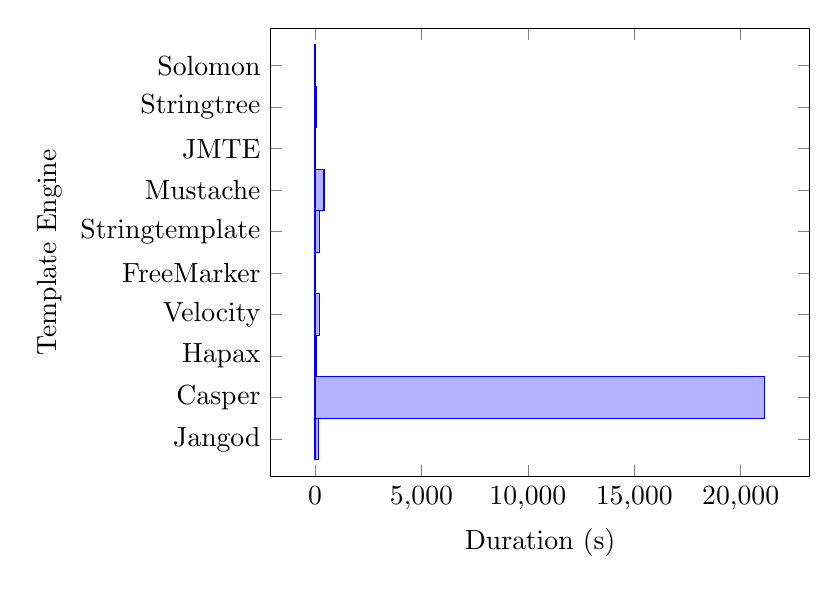
\begin{tikzpicture}
\begin{axis}[
    scaled ticks=false,
    % xmode=log,
    % ticks with fixed point,
    % scaled ticks=false,
    xbar stacked,
	bar width=15pt,
	% nodes near coords,
    ytick=data,
    legend style={at={(0.5,-0.20)},
      anchor=north,legend columns=-1},
    ylabel={Template Engine},
    xlabel={Duration (s)},
    symbolic y coords={
        Jangod, Casper, Hapax, Velocity, FreeMarker,
        Stringtemplate, Mustache, JMTE, Stringtree, Solomon
    },
    ]
\addplot+[xbar] plot coordinates {
  (180.5,Jangod) (21138.3,Casper) (73.6,Hapax) (196.6,Velocity) (29,FreeMarker)
  (196.6,Stringtemplate) (418.8,Mustache) (17.4,JMTE) (86.5,Stringtree) (8,Solomon)
};
\end{axis}
\end{tikzpicture}
\caption{Mean test duration by template engine}
\label{fs:graph:duration}
\end{figure}

\begin{figure}[ht]
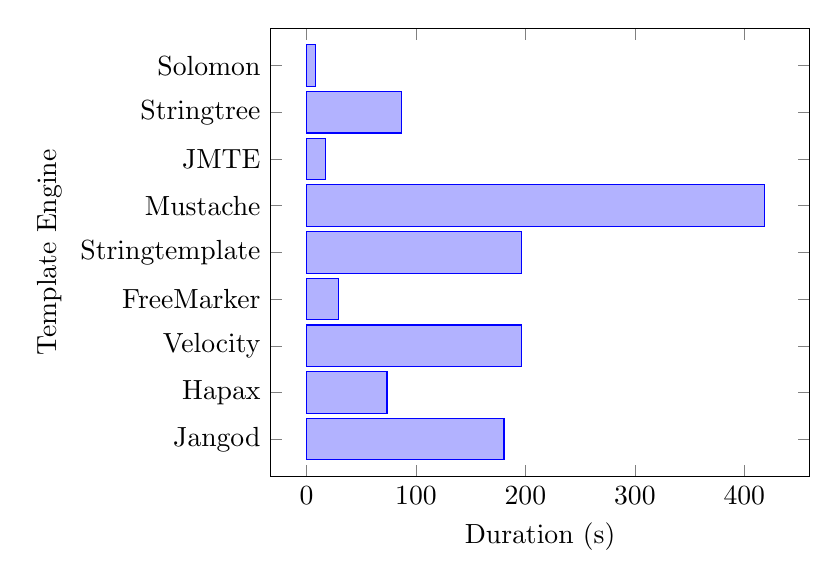
\begin{tikzpicture}
\begin{axis}[
    scaled ticks=false,
    % xmode=log,
    % ticks with fixed point,
    % scaled ticks=false,
    xbar stacked,
	bar width=15pt,
	% nodes near coords,
    ytick=data,
    legend style={at={(0.5,-0.20)},
      anchor=north,legend columns=-1},
    ylabel={Template Engine},
    xlabel={Duration (s)},
    symbolic y coords={
        Jangod, Hapax, Velocity, FreeMarker,
        Stringtemplate, Mustache, JMTE, Stringtree, Solomon
    },
    ]
\addplot+[xbar] plot coordinates {
  (180.5,Jangod) (73.6,Hapax) (196.6,Velocity) (29,FreeMarker)
  (196.6,Stringtemplate) (418.8,Mustache) (17.4,JMTE) (86.5,Stringtree) (8,Solomon)
};
\end{axis}
\end{tikzpicture}
\caption{Mean test duration excluding Casper}
\label{fs:graph:duration-excluding}
\end{figure}

\section{Analysis}
\label{fs1:analysis}

It is reassuring that all the template systems in the study were capable of processing both plain text (S0) and simple substitution (S1) cases. However, these were the only scenarios which everything passed. For all the other test scenarios there was at least one template engine which could not manage it. There were only four template engines in the sample which correctly rendered every scenario: \emph{Solomon}, \emph{Stringtree}, \emph{Freemarker}, and \emph{Casper}. Given that these scenarios were chosen as representative of common situations in professional software development, it is surprising that there was so much variability in features. The documentation for all the implementations makes some kind of claim of being `powerful', `flexible' or `suitable for a wide range of projects'. 

Consider, for example, the \emph{Hapax} template system which failed five of the eight tests. Its documentation states:

\begin{displayquote}
Hapax is a simple but powerful text templating library for Java. Hapax is suitable for constructing text output from Java code. The syntax is similar to Google's ctemplate library, and emphasizes the separation of logic from presentation. Hapax was designed to be easy to use and have minimal dependencies. Hapax does not depend on any existing web framework, and is suitable for use in servlets, scripting languages (Scala, Groovy, etc), and server-side applications.
\end{displayquote}

Nowhere in this does it mention any limitations, making comparing implementations on documentation alone a tricky proposition. Attempts have been made to compile comparative lists of such software by features \citep{Wikipedia2018} but interpretation of the exact meaning of each feature can be loose, and there would potentially be great benefit in defining a comprehensive set of such benchmark scenarios which could be used to compare and evaluate even software which is not found in such lists. The production of such benchmark scenarios would be difficult, however, because of the wide differences between template languages. There is currently no single `meta language' in which scenarios can be expressed for multiple template engines. This problem is explored further in \autoref{chapter:intermediate}.

In many cases the limitations of the template engines seem closely tied to the choice of template language. The minimalist language common to many \emph{Mustache} implementations, for example, deliberately avoids constructs such as loops, in favour of performing such logic in application code before invoking the template engine. While this can be a workable strategy, and satisfies \citeauthor{Parr2004}'s (\citeyear{Parr2004}) desire for separation of concerns between view and model, it also has some potential drawbacks. Preparing values requires extra processing in the application code, which partially disguises the processing cost of generating pages compared to more competent template engines. It also requires that every possible configuration of data for the page is pre-calculated, including `expanding' collections. While expanding lists of textual or numeric values is relatively simple, this approach becomes much more complex in the relatively common case where each entry in the list needs to be processed using a template in order to display the result. This approach also denies the template engine any possibility of automatically re-using intermediate values or using `lazy evaluation' strategies to avoid unused calculations, for example when Boolean conditions remove the need for a value to be rendered. Such choices have considerably more impact when the same application code is used to evaluate a wide variety of templates, each with different data requirements. In common with many software development habits, which prioritise development effort over execution time, it can be easier for developers to produce general-purpose code which pre-calculates everything required by every possible template, even though many of those values will not be required for any given rendered page. This can add extra, unneeded, processing cost to every page.

There is also an anomaly in the timings. In table 3.2, it appears that several of the template engines take longer to process a plain text file than a simple substitution. While this is possible, it seems somewhat unlikely, so the experiment was temporarily adjusted to run the tests in a different order. Whichever test runs first seems to take longer. The current hypothesis is that this is an artefact of some kind of “warm up” behaviour, either in the template engine code or in the Java language and runtime. This implies that the data in table 3.2 should not be used to compare performance across scenarios for any given template engine, but the the experiment remains useful for comparing the range of performance between template engines.

The software `test bench' for these measurements was constructed using the strategy pattern (as shown in \autoref{fs:figure:strategy}) with all the template engine libraries loaded into memory at the same time. This made running the experiments much simpler, as they could be performed by a simple loop through a collection of \emph{TemplateSystem} objects with no need to stop or start the code, or to add and remove external code blocks. However, this approach also required some careful coding to deal with potential clashes and incompatibilities between the separate template libraries and their transitive dependencies. The version of Java used for these experiments did not provide any form of separation between libraries beyond class and package names. Any problems with any of the template engine implementations (such as a syntax error in a template specification) which caused the template engine to `crash' or raise an exception, would abort the whole test run. It is not clear whether there was any more subtle interference between the separate libraries which may have affected the results.

The approach of treating this code as a `throw away' experiment and writing only the minimum code necessary to perform the experiments had an impact on the usability of the software. Result values were simply printed out as soon as they were calculated, without performing any analysis or data formatting. This required manual copying into analysis software to determine derived results such as the mean duration. Configuration parameters such as the collection of template engines to be tested and the number of times to invoke them were hard-coded into the software, which meant that any change required editing and re-compliation of the experiment code.

Finally, it is important to note that this feasibility study only measured two things: the ability to correctly render some specific scenarios, and the time taken to perform them. While some \emph{guesses} may be made about what that might mean for overall energy usage, this study does not say anything definitive about the energy usage of the different template engines.

Further research is needed to address the above issues. Methods of measuring the energy usage of software are explored in \autoref{chapter:testrig} .Improvements to the construction and operation of the test framework and the measurement of the energy usage of components are discussed in \autoref{chapter:fs2}.

\subsection{Analysis of Individual Template Engines}

It is clear from \autoref{fs:table:times} that performance of different template engines varies widely. Examining the code of the outliers (\emph{Solomon}, the fastest, and \emph{Casper}, the slowest) shows some interesting features. Casper has obviously been designed to be as flexible as possible, going so far as to start a complete JavaScript interpreter for every page generated, and discarding it when the page is completed. This imposes a relatively huge burden on generating regular web pages but does potentially provide some facilities unavailable in most other systems. It is important to note that this feasibility study was designed based on common web page scenarios, and thus does not include any cases where Casper would be the only applicable solution. Solomon, on the other hand has been coded solely for speed. It uses a relatively non-standard template language, optimised for simple and fast processing rather than easy readability. One other template engine in this study (\emph{Stringtree}) uses a similar template language to Solomon but does not achieve the same performance benefits. When Stringtree was coded, performance was not the primary goal.

One template engine, \emph{Casper}, takes so long to perform the experiments that it makes \autoref{fs:graph:duration} unusable for comparing the performance of the other template engines. By removing Casper from the results (see \autoref{fs:graph:duration-excluding}) a more nuanced view of their relative performance can be seen. In this figure, template engine performance can be seen to cluster into a few groups. \emph{Mustache} is in a group of its own, at over 400s, taking roughly twice the time as the engines in the next group. The next group contains three template engines: \emph{Stringtemplate}, \emph{Velocity}, and \emph{Jangod} all of which take around 200s. A third group includes \emph{Hapax} and \emph{Stringtree} which both take a bit less than 100s to complete the run. The final, fastest, group includes \emph{Solomon}, \emph{JMTE}, and \emph{Freemarker}, all taking 30 seconds or less.

If the above experiments were used to select a template engine for a project based on performance, then the three template engines in the fastest group would form the short-list. Selecting between these three would then depend on further factors. \emph{Solomon} is clearly the fastest, and it is able to correctly perform all the scenarios, so is the obvious choice. However, Solomon uses a slightly unusual template language which could hinder adoption. JMTE is the second fastest, but could not correctly perform all the scenarios. In development situations where the missing features are not important, however, then JMTE could be a good compromise. \emph{Freemarker}, although it is up to 18 times slower than Solomon for some cases, was the only popular template engine to correctly perform all the scenarios. FreeMarker also has the advantage of a well-documented template language and wider adoption than the other two, so would also make a good choice for a more conservative development team. Based on their performance it would seem a poor choice to select any of the others.

\section{Discussion and Initial Conclusions}
\label{fs:discussion}

\subsection{Discussion}

A key finding to arise from the feasibility study is the surprising variety in capabilities and performance between purportedly similar software libraries. For some common operations in this study there was over 10,000 times difference between the best and the worst performers. Even averaged across the range of different operations, the difference in time taken to perform the same task is still over 2,500 times between the best and worst performing libraries.

Such stark contrast is nowhere to be found in the documentation, however, which makes selecting a template engine for use in a software project a difficult task. All the components evaluated in this study are free software, so the traditional approach of minimising the purchase cost does not apply. All the components are available with licences which permit inclusion in commercial software, so considering licence terms is also no use in selecting between them. Despite their free availability, and with no direct financial incentive to increase `sales', they often provide documentation which reads like optimistic and unsubstantiated advertising copy. Such documentation as is provided tends to concentrate on listing and describing specific available features, covering everything else with blanket subjective statements such as `fast', `powerful' or `flexible'. This paucity of information leaves makes it hard for developers to make informed choices.

The fact that one template engine, \emph{Solomon}, was able to correctly perform all the scenarios in a much faster time than any of the others when they are all written in the same programming language and running on the same platform, shows that the choices made in the design and programming of the different template engines in this study have had a huge impact on the performance and capabilities of these supposedly equivalent components. In this specific case, one reason could be that \emph{Solomon} was written to minimise multiple handling of template characters. Whenever possible, input characters are passed directly to the output document without buffering. The characteristics of the \emph{Solomon} template language (discussed in more detail in \autoref{section:comp:languages}) help reduce the need for buffering.

\subsection{Feasibility Study Conclusions}

In conclusion, preliminary results show that there is a surprisingly wide range of difference in capabilities and performance between superficially similar solutions to a specific class of problem. The study provides data which was not clear from the on-line documentation for the components being considered. This in turn suggests that a change in software development behaviour, both when writing software and when selecting components or libraries, could potentially make a noticeable difference in overall energy and resource usage of large software systems such as the world wide web. Further research is required to explore and quantify this impact.

In particular, the following specific conclusions will be taken forward from this feasibility study:

\begin{itemize}
\item The differences between this sample of components are large enough to be worth proceeding with the research.
\item Choices made during design and development of software, and when selecting components, can have a large impact on the performance of the final product.
\item The methodology of constructing a range of representative scenarios and using them to compare the different components is fundamentally sound, however, improvements are needed to the implementation of the tests
\item The template languages used by the different template engines vary widely enough that further research is needed on ways to simplify the creation of equivalent templates for a range of template engines.
\item Further research is needed to determine what impact this wide variety in performance might have on energy usage.
\end{itemize}
